The temperatures in silicon detector systems are critically important to their performance. Fundamentally, the leakage current of a silicon sensor has a pronounced temperature dependence 
\begin{equation}
I\propto T_\text{S}^2e^{-T_\text{A}/T_\text{S}},
\label{eq:leakage_current_temp_dependence}
\end{equation}
where $T_\text{S}$ is the sensor temperature and $T_\text{A}\simeq7000$~K. Leakage currents can become particularly significant after irradiation of the silicon material. The heat generated by these leakage currents in the silicon sensor, together with the heat from front-end electronic components on the detector, needs to be removed by a cooling system. The capability of the cooling system to remove this heat is limited by the temperature of the local cold sink (typically a circulated fluid) and the thermal impedance of the heat path between the source (electronics and sensor) and the sink. Due to the strong growth of leakage power with temperature, there is a critical temperature $T_\text{crit}$ above which the heat cannot be removed quickly enough, and the detector becomes thermally unstable (`thermal runaway')\footnote{In a real detector system, the resulting growth of sensor temperature would be arrested by overcurrent limits in the power supplies, resulting in a reduction of the bias voltage. At the same time, the increased current leads to an increase of the noise, such that the overall result is a degradation of the S/N performance of the system.}. It therefore crucial to understand the thermal behaviour of the detector system in order to avoid the conditions of thermal runaway. Even before the limit of thermal stability is reached, knowledge of temperatures in silicon detector systems is important, as they determine
key system parameters such as power supply capacity and cable dimensions.

In addition to the silicon,
there can be aspects of the front-end electronics that have a temperature dependence. In the strip system for the ATLAS Phase-II upgrade \cite{Collaboration:2017mtb}, which is the subject of this case study, there are two additional temperature-dependent heat sources. The first is a radiation damage effect in the readout electronics, which leads to an increase in the digital power of the chip whose magnitude depends on the total ionisation dose (TID) and the temperature of the chip \cite{Collaboration:2017mtb}. This phenomenon was first observed in the ATLAS IBL \cite{ATL-INDET-PUB-2017-001}. The other temperature dependence of a power source stems from the converter chip (FEAST \cite{1748-0221-6-11-C11035}) used in the on-detector DC-DC converter system supplying power to the front-end electronics. 


In principle, the temperatures in the system for a given set of operational parameters (power density, thermal conductivities, etc.) can be predicted by FEA to an accuracy that is limited only by the quality of the input parameters. However, this is a time-consuming process and can be prohibitively difficult if a number of local heat sources depend non-linearly on temperature. A simplification to this problem that allows for an analytical solution in the case of a simple heat source topology has been developed in~\cite{Beck:2010zzd}. Here we develop this method further to include several temperature-dependent non-linear heat sources in the front-end electronics. The resulting set of equations cannot be solved analytically anymore, but the solution can be found with little effort using numerical problem solvers. This enables us to predict with some confidence the temperatures and power requirements in the ATLAS strip system throughout Phase-II operation. The results from this prediction have been used throughout the project to consistently dimension the different systems (cooling, power, services, etc.), with some additional margin due to the inclusion of a common set of safety factors. This method can be easily adapted to any other system by adjusting the model to the system-specific geometries and parameters.

\subsection{The ATLAS strip system}
The strip system for the ATLAS Phase-II upgrade \cite{Collaboration:2017mtb} consists of two parts: the barrel system, comprised of four concentric cylindrical barrels, and two endcaps consisting of six disks each.

In the barrel, the detector modules are made of square sensors ($96.85\times 96.72$~mm$^2$) with a hybrid on top, which hosts the front-end chips (ABC130 \cite{abc130} and HCC \cite{Collaboration:2017mtb}) as well as circuitry to convert the supply voltage of larger than 10~V to the chip voltage of 1.5~V. This circuitry is controlled by the FEAST chip. The modules are glued onto both sides of a composite sandwich that contains two parallel thin-wall titanium cooling pipes embedded in carbon foam (Allcomp K9 - ref)  between two facesheets of UHM carbon fibre (3 layers of K13C2U/EX1515) with a co-cured Kapton/copper low-mass tape. A model of this geometry is shown in Fig.~\ref{fig:barrelgeometry}. During final operation, cooling will be achieved by evaporating CO$_2$ in the cooling pipes with a final target temperature no higher than $-35^\circ$C anywhere along the stave.

The geometry of the stave is uniform along its length, with the exception of the end region of the stave, where an End-Of-Structure (EOS) card is mounted on both surfaces. The EOS card shares part of its heat path with the module; underneath the EOS, the thermal path is degraded by the presence of electrically-insulating ceramic pipe sections. The thermal and electrical properties of a module adjacent to the EOS card (hereafter refered to as an `EOS module') are sufficiently different from other modules along the lenth of the stave (`normal modules') to warrant separate treatment in the thermo-electric model of the barrel.

\begin{figure}[ht]
\centering
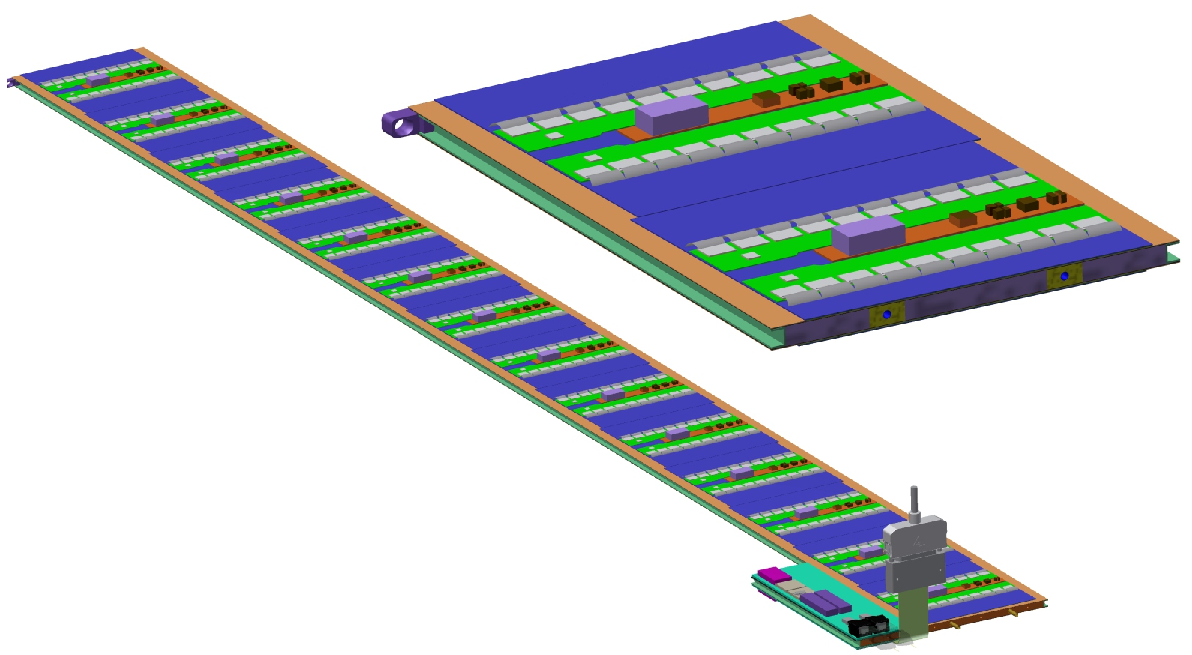
\includegraphics[width=0.8\linewidth]{figures/stave.pdf}
\caption{Strip barrel local support geometry. On the left, a complete stave is shown (EOS card in the foreground). The right picture shows a cross-section of the stave with the two cooling pipes visible inside the core. }
\label{fig:barrelgeometry}
\end{figure}

The endcap system consists of two endcaps composed of 6 disks each.
Each disk contains 32 `petals,' the local substructure depicted in Fig.~\ref{fig:endcapgeometry}.
Both sides of the petal are loaded with 6 silicon modules, each with a distinct design,
located at increasing radius from the beam pipe and labeled R0 through R5 (where `R' stands for ring).
Each endcap module consists of one
or two irregularly-shaped silicon sensors, and a varying number of front-end chips and DC-DC converters on each module.
% (between 12 and 28 ABCs, and 2 to 4 HCCs).
The EOS card is located adjacent to the R5 module, but the
cooling pipes run directly underneath it without a shared heat path, in contrast to the barrel EOS.
The remaining module and petal core design details are largely identical to the barrel module description above.

\begin{figure}[ht]
\centering
%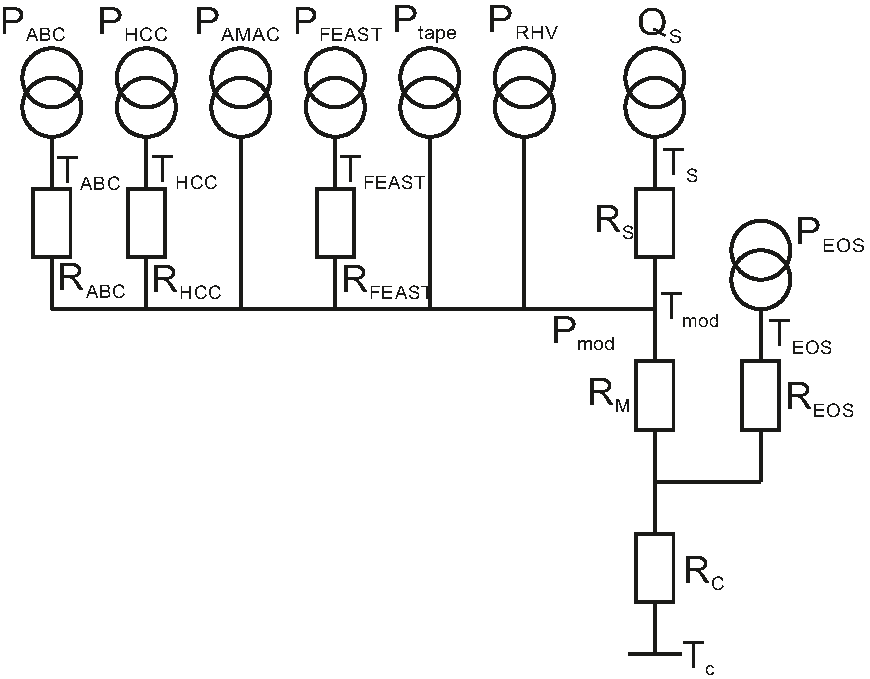
\includegraphics[width=0.6\linewidth]{figures/Thermalmodel.pdf}
\caption{Endcap strip geometry}
\label{fig:endcapgeometry}
\end{figure}

\subsection{Radiation environment}
A key input to the calculation is the radiation environment of the strip system, as several inputs depend on radiation damage effects. The sensor leakage current can be parametrized as  a function of the fluence expressed in 1~MeV neutron-equivalents, and the TID effect on the digital chip current will be described as a function of the total ionizing dose rate (more details on its dependencies can be found in Section~\ref{fig:feast_eff}). 

Predictions for both of these parameters for each point in the ITK are available which have been generated using the FLUKA particle transport code and the PYTHIA8 event generator (Fig.~\ref{fig:radiation}) \cite{background}. Both of these distributions display a weak dependence on $z$ in the barrel, whereas they vary significantly along $r$ and $z$ over the length of the endcap petals. Because of this, and the linear uniformity of the stave compared to the more complex geometry along a petal, we modelled only two types of modules for the barrel (a generic module along the linear part of the stave and the module next to the end-of-structure card), but six different types of modules in a petal.
% Note here: the fluence is a justification for modeling layer 0-3 separately, and using
% the flux/TID to model 6 separate versions of a petal.
% The module design justifies 2 (6) different module types in the barrel (endcap).

\begin{figure}[ht]
\centering
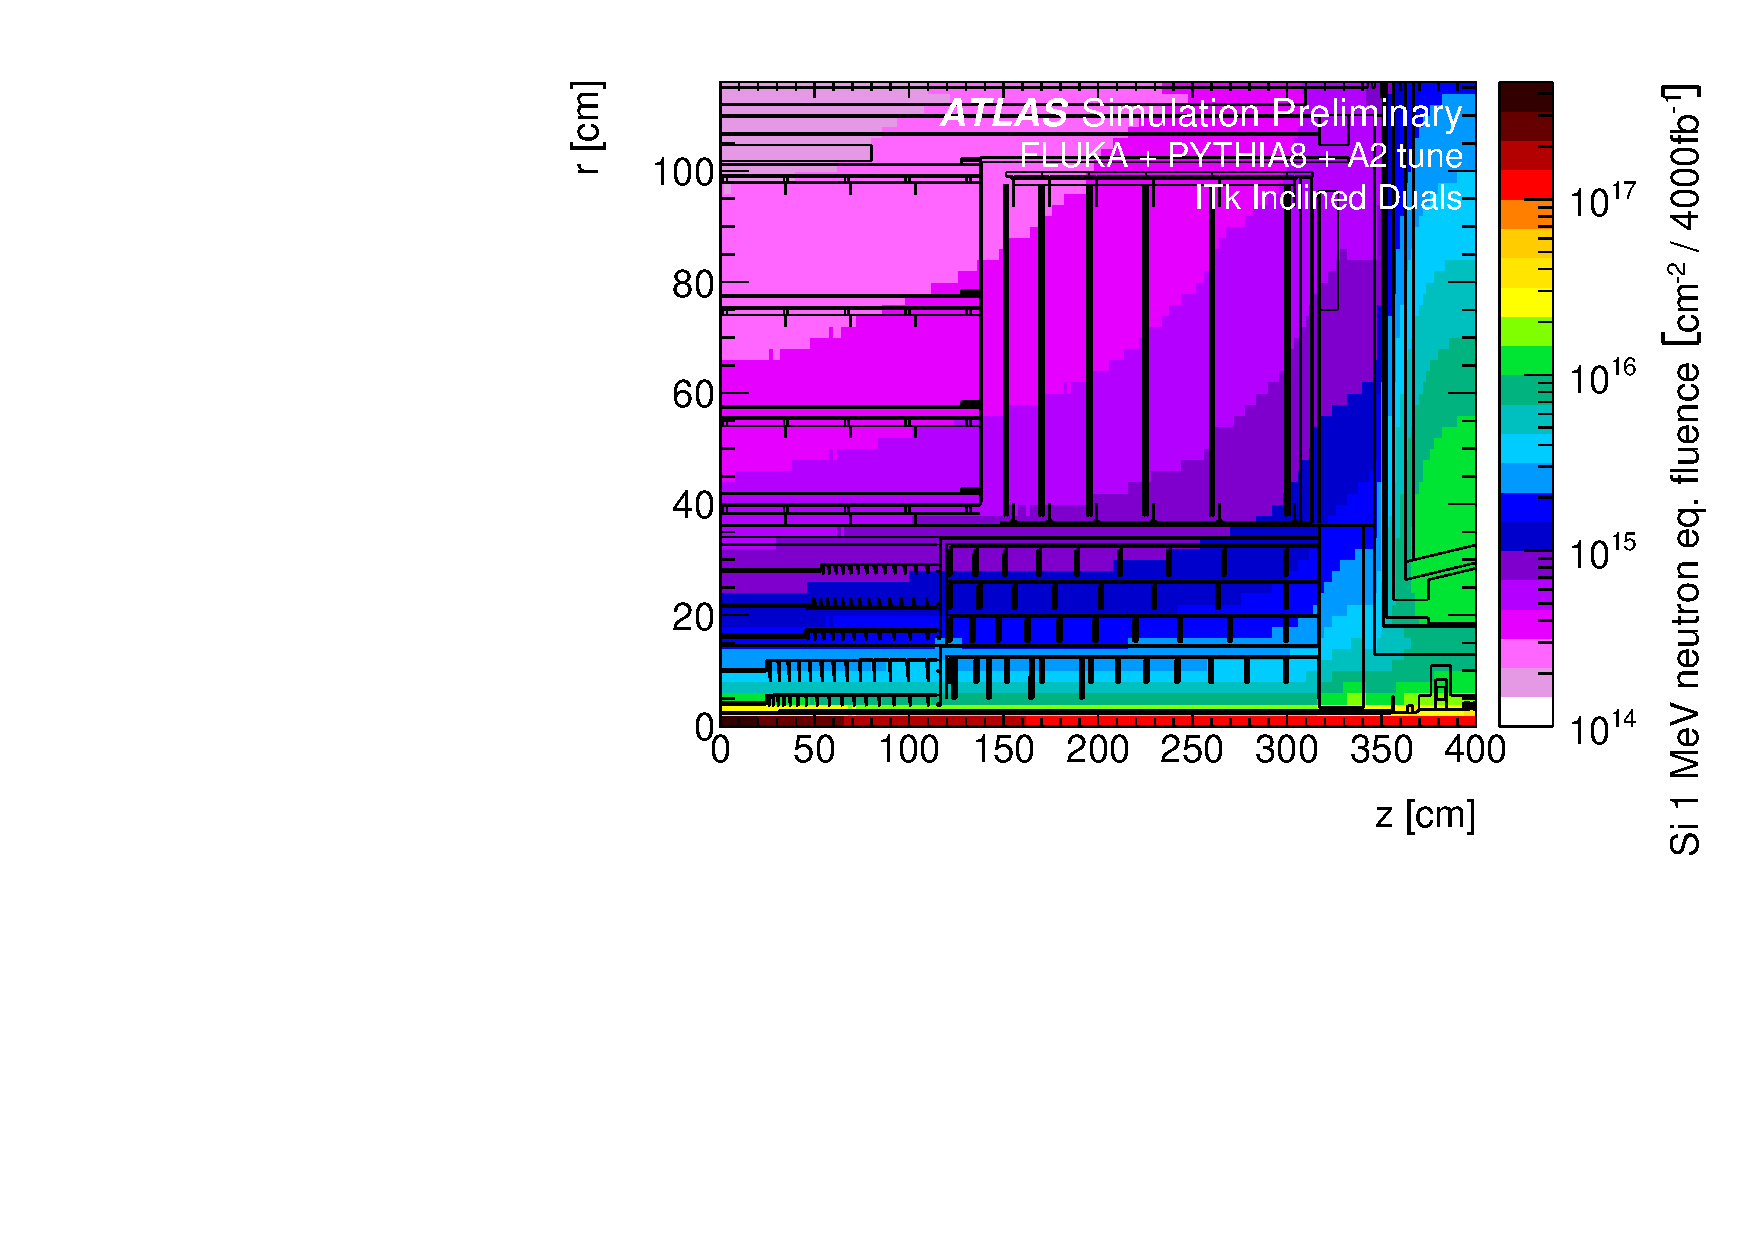
\includegraphics[width=0.48\linewidth]{figures/fluence.pdf}\quad
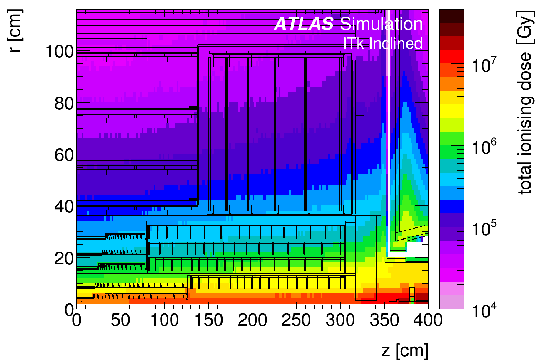
\includegraphics[width=0.48\linewidth]{figures/TID.pdf}
\caption{ATLAS ITk radiation environment. 1~MeV neutron equivalent fluence (left) and total ionizing dose (right). Both plots are for an integrated luminosity of 4000~fb$^{-1}$ \cite{background}.}
\label{fig:radiation}
\end{figure}
